\chapter{Reporting Errors}
\label{user-errors}

If \FramaC crashes or behaves abnormally, you are invited to report an issue
\via the \FramaC Gitlab repository, located at \url{https://git.frama-c.com}.
The {\em New Issue} page (\url{https://git.frama-c.com/pub/frama-c/issues/new})
allows creating a new report, but you will need an account.

\begin{important}
  Unless you have an account provided by the \FramaC team, you need to sign in
  using a Github account, as shown in Figure~\ref{fig:gitlab-login}.
\end{important}

\begin{figure}[htbp]
\begin{center}
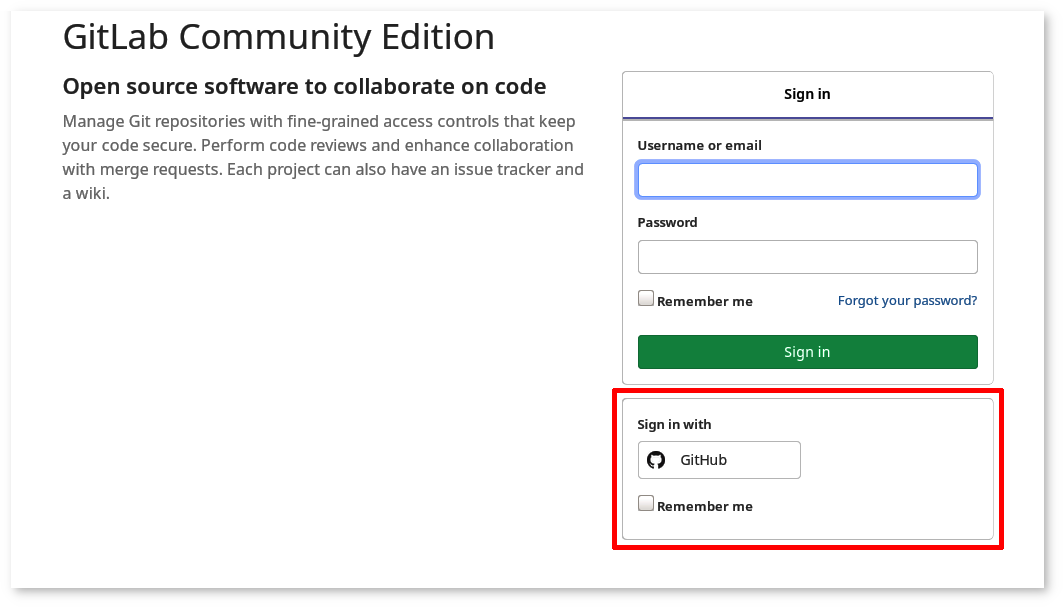
\includegraphics[width=\textwidth]{gitlab-login.png}
\end{center}
\caption{The \FramaC Gitlab login page. Note that no direct account creation
  is possible; you need to sign in via Github unless the \FramaC team
  provided you an account.}
\label{fig:gitlab-login}
\end{figure}

When creating a new issue, choose the \texttt{bug\_report} template next to
{\em Title}, then enter the title and fill the template.

Bug reports can be marked as public or confidential.
Public bug reports can be read by anyone and may be indexed by search
engines. Confidential bug reports are only shown to \FramaC developers.

Reporting a new issue opens a webpage similar to the one shown in
Figure~\ref{fig:gitlab-bug-report}.
\begin{figure}[htbp]
\begin{center}
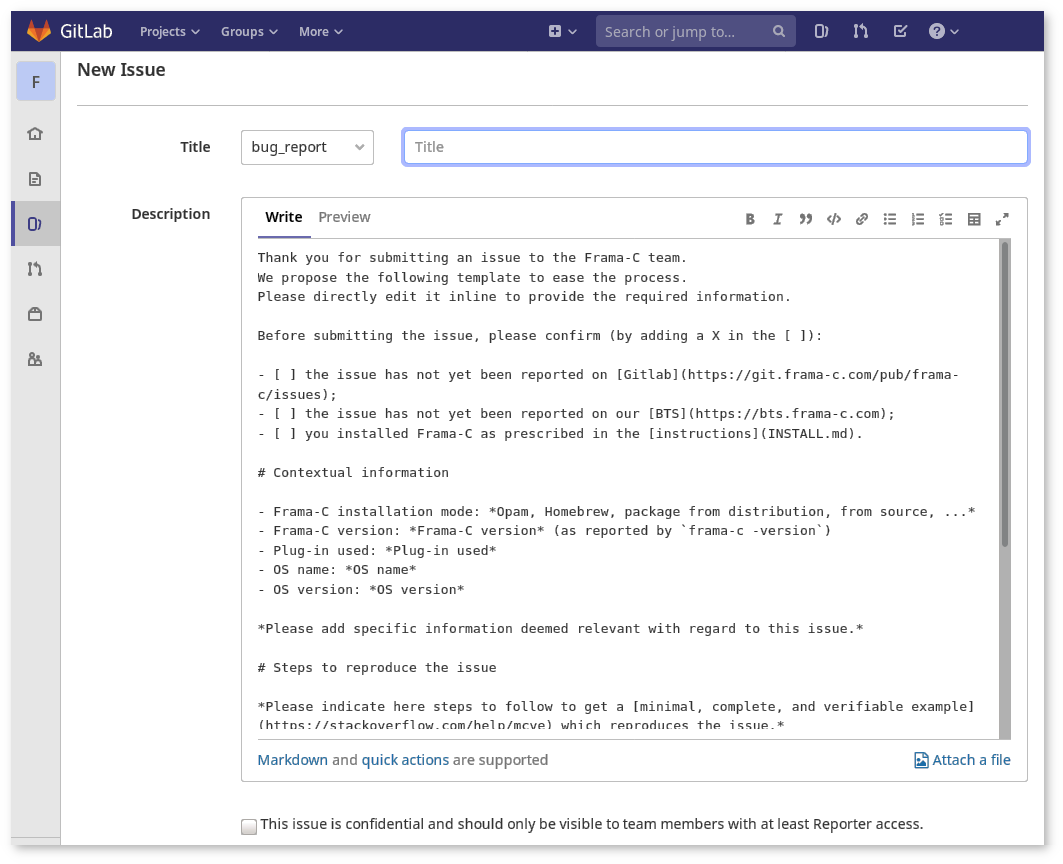
\includegraphics[width=\textwidth]{gitlab-bug-report.png}
\end{center}
\caption{The Gitlab new issue page, with the \texttt{bug\_report} template.
  The checkbox at the bottom enables marking the issue as private, so that
  only \FramaC developers can see it.}
\label{fig:gitlab-bug-report}
\end{figure}

Please fill the template as precisely as possible,
\emph{in English}\footnote{French is also a possible language choice for
  private entries.}, which helps the \FramaC team more quickly understand,
reproduce and respond to the issue. The form uses Markdown syntax and you can
attach source files and screenshots to the issue.

Replies and updates concerning your issue are sent by e-mail by Gitlab.

%% Local Variables:
%% compile-command: "make"
%% TeX-master: "userman.tex"
%% ispell-local-dictionary: "english"
%% End:
